\chapter{Fejlesztői dokumentáció}
\label{ch:impl}

Ebben a fejezetben a szoftver működését részletezem.
Például szoftver felépítésére, a szoftverben használt tervezési mintákra és
a fontosabb algoritmusok működésére is kitérek.
A szoftver forráskódja a jövőben változhat,
a frissített API dokumentáció ezért a személyes oldalamon is elérhető \cite{apidoc}.

\section{Csomagok és modulok}

A szoftver forráskódja több csomagban és modulban található.
A forrráskód jelentős része öt fő csomagba van szerveze,
ezek az alábbi táblázatban láthatók.

\begin{table}[H]
	\centering
	\begin{tabular}{ | m{0.25\textwidth} | m{0.65\textwidth} | }
		\hline
		\textbf{Csomag} & \textbf{Rövid leírás} \\
		\hline \hline
		\emph{app} & GUI alkalmazás csomagja \\
		\hline
		\emph{client} & adatbázis kliens \\
		\hline
		\emph{model} & adatok modellezése és mentése \\
		\hline
		\emph{tests} & egység és egyéb tesztek \\
		\hline
		\emph{transformations} & átalakítások forráskódja és API az átalakításokhoz \\
		\hline
	\end{tabular}
	\caption{A szoftver fő csomagjai}
	\label{tab:packages}
\end{table}

A fő csomagok (a \emph{tests} csomag kivételével) nem tartalmaznak "futtatható" fájlokat,
a belépési pontok külön modulokba vannak szervezve.

\begin{table}[H]
	\centering
	\begin{tabular}{ | m{0.25\textwidth} | m{0.65\textwidth} | }
		\hline
		\textbf{Modul} & \textbf{Rövid leírás} \\
		\hline \hline
		\emph{launch} & GUI alkalmazás belépési pontjának modulja \\
		\hline
		\emph{persistor} & CLI program belépési pontjának modulja \\
		\hline
		\emph{utils} & utility függvények modulja (pl. fájlok olvasásához)  \\
		\hline
	\end{tabular}
	\caption{A szoftver fő moduljai}
	\label{tab:modules}
\end{table}

\section{A \emph{client} csomag}

A \emph{client} csomag feladata az adatbáziskapcsolat és az indexek létrehozása.
A kliens a \emph{pymongo} könyvtárat használja, implementációja a \emph{Client} osztályban van.
Ha szoftvernek az adatbázisra van szüksége azt ezen az osztályon keresztül érheti el.
Például az adatbázis forráskódokat és forráskód-párokat tartalmazó kollekciói a kliensen
keresztül elérhetők.

A \emph{Client} osztály a Python-ban gyakori \emph{monostate} \cite{monostatePattern}
tervezési mintát használja, a minta a \emph{singleton}-hoz hasonló,
de a több példány létrehozását is megengedi.
Egy \emph{monostate} osztálynak van egy belső (statikus) állapota,
példányosításnál ezt a belső állapotot adja vissza.
Ez hasznos, mert a példányok egy közös állapoton osztoznak, ami a program több részéről is elérhető.

Python-ban az objektumok állapota reprezentálható egy dict segítségével,
ezért a \emph{monostate} mintát nagyon egyszerű implementálni:
a belső állapot egy dict lesz, példányosításnál a belső állapot dict-je alapján létrehozunk egy objektumot.

\begin{figure}[H]
	\centering
	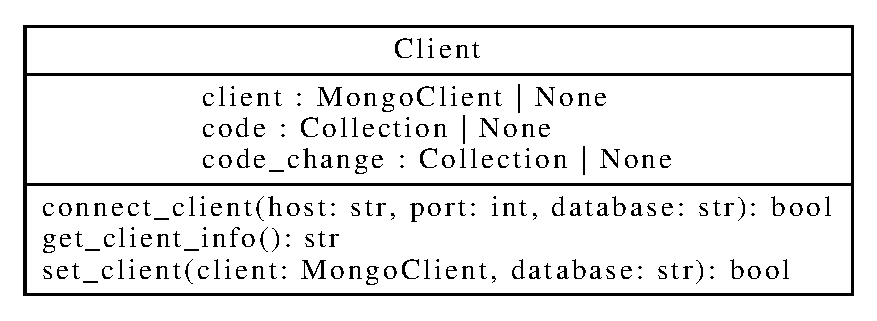
\includegraphics[width=0.6\textwidth]{images/uml/Client.eps}
	\caption{A \emph{Client} osztály UML diagramja}
\end{figure}

Amikor először példányosítunk a \emph{Client}-ből a \emph{client}, \emph{code} és \emph{code\_change}
attribútumai \emph{None} értékeket vesznek fel (ez a kezdelteges belső állapot).

Ha ezután meghívjuk a \emph{connect\_client} metódust az adatbázis paramétereivel
és a kapcsolat 10 másodpercen belül létrejön, akkor a kapcsolat sikeres.
Ekkor
a \emph{client} attribútum az adatbáziskliens,
a \emph{code} és \emph{code\_change} attribútumok pedig rendre
a kódokat és kód-párokat tartalmazó kollekciók lesznek.

A kollekciók akkor is létrejönnek a kliens szintjén ha az adatbázisban még nem szerepelnek.
Ebben az esetben a kollekció az adatbázisban akkor jön létre ha a kliensen keresztül elmentünk egy dokumentumot.
A kliens a szükséges indexeket is definiálja.

\section{A \emph{model} csomag}

A \emph{model} csomag a feladata a forráskód-párok modellezése, három modulból áll:

\begin{itemize}
	\item \emph{datatypes} - az adattípusokat definiáló modul
	\item \emph{serializers} - az adattípusokat szerializáló modul
	\item \emph{stores} - az adattípusokat elmentő modul
\end{itemize}

A csomagban két adattípust definiálok a \emph{Code} és \emph{CodeChange}.
A \emph{Code} a forráskódok modellje, a \emph{CodeChange} pedig a forrráskód-párokat modellezi.

\begin{figure}[H]
	\centering
	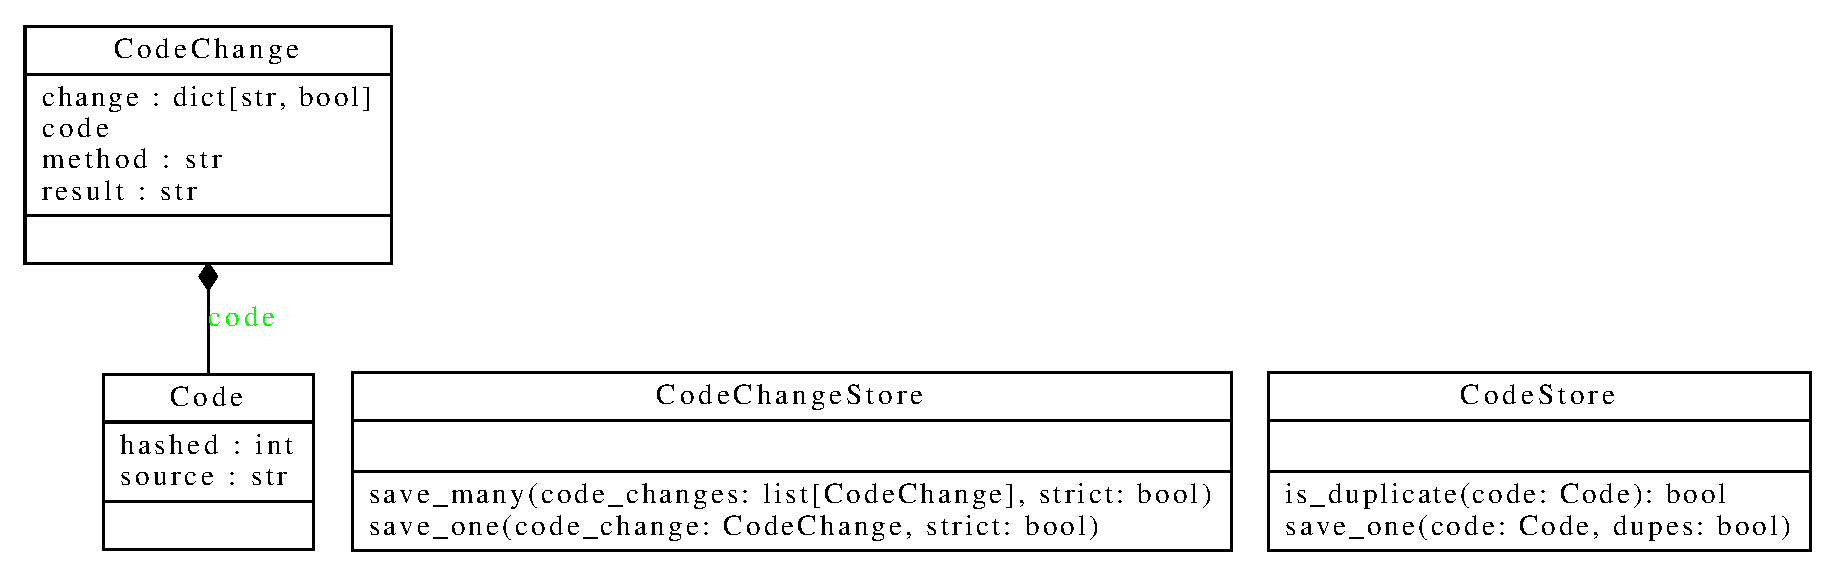
\includegraphics[width=0.9\textwidth]{images/uml/modells.eps}
	\caption{A model csomag osztályainak UML diagramjai}
\end{figure}

A forráskód a duplikátumok kiszűrése miatt rendelkezik saját modellel.
A duplikált forráskódok szűrése azért szükséges, mert GitHub-on a kódok jelentős része duplikátum
\cite{gitubDuplication},
vagyis ha GitHub-ról bányászunk kódokat akkor a generált adathalmaz minőségén javíthatunk,
a duplikátumok kiszűrésével.

A kódok modellje ezért a kód mellett a kód \emph{sha256}-os hash-ét is tárolja.
Mielőtt a kódot elmentjük az adatbázisba megnézzük, hogy a hash ütközik-e.
A hash attribútum indexelve van a kódokat tartalmazó kollekcióban, ez biztosítja a gyors lekérdezést.
Ha nincs ütközés, akkor a kódot egyből hozzáadhatjuk az adatbázishoz,
ha vannak ütközések, akkor csak az ütköző kódokat kell összehasonlítani.

A duplikátumok kiszűrését a \emph{CodeStore} osztály \emph{save\_one} metódusa végzi,
a \emph{CodeChangeStore} osztály segítségével pedig a kód-párokat tartalmazó kollekcióba
szúrhatunk be dokumentumokat.

A \emph{CodeStore.save\_one} metódusában a duplikátumok szűrése opcionális,
tehát ha duplikátumoktól mentes kódokból is generálhatunk adathamlazt ha szeretnénk.

\section{Az \emph{app} csomag}

Az \emph{app} csomag feladata az átalakításokat szemléltető GUI-s alkalmazás megvalósítása.
Az alkalmazás architektúrája modell-nézet-kontroller (MVC) szerű.
Egy nézet rendelkezik egy kontrollerrel és a kontroller pedig egy modellel.

A nézet feladata a GUI definiálása és frissítése,
a modell feladata az adatelérés vagy az alkalmazás állapotának modellezése.
A kontroller ezt a két réteget köti össze,
így a nézet nem függ a modelltől és a modell sem a nézettől.

Az alkalmazás csomagjainak UML diagramját az alábbi ábrán láthatjuk.

\begin{figure}[H]
	\centering
	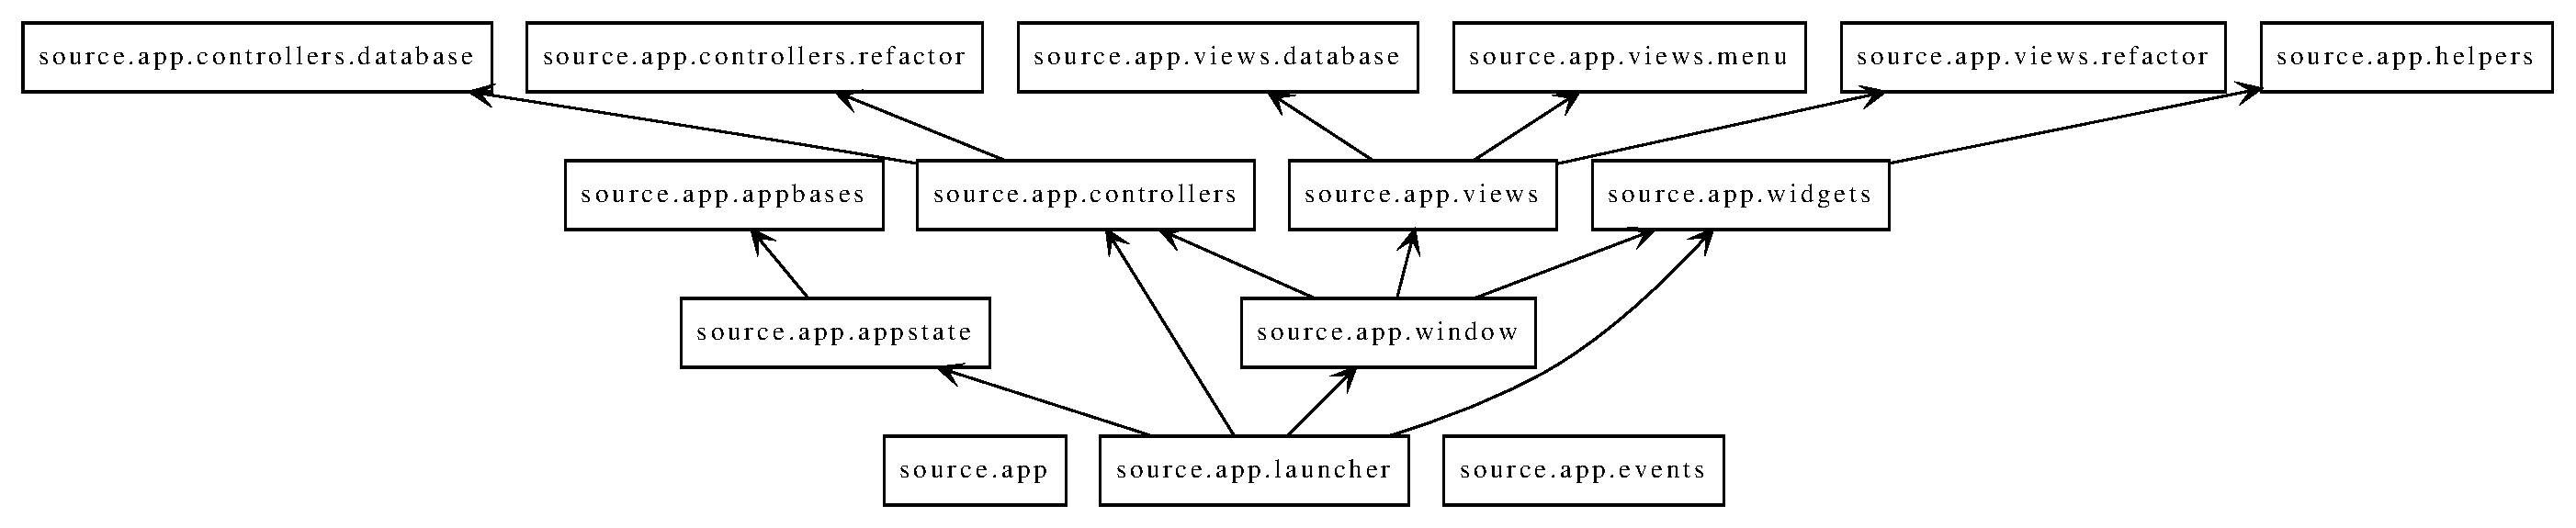
\includegraphics[width=0.9\textwidth]{images/uml/apppackages.eps}
	\caption{Az alkalmazás csomagjai}
\end{figure}

\subsection{Állapotmodell}
\label{subsec:appstate}

Az alkalmazásban kétféle modell különböztethető meg:
az adatelérési modellek, amik működéséről az előző szekcióban olvashatunk
és az alkalmzás állapotmodellje ami az \emph{app.appstate} modulban található.

Az állapotmodell az \emph{AppState} osztályban van definiálva és 
az \emph{observer} tervezési mintát használja a nézetek frissítésére.
Az \emph{AppState} osztály az \emph{Observable} osztályból származik,
ezért rendelkezik megfigyelők (\emph{observers}) egy listájával,
ami esemény-eseménykezelő párok listája.

Ha a nézet egy komponenesét az állapotmodell változásának hatására szeretnénk frissíteni,
akkor azt az eseménykezelőt, ami frissíti, hozzárendelhetjük az állapotmodell egy
eseményéhez az \emph{app.events} modulból.

Hozzárendelni egy eseménykezelőt egy eseményhez az \emph{Observable} osztály
\emph{attach} metódusával lehet.
Ha az adott eseményt kiváltja egy változás a modellben, akkor a modell értesíti a
nézeteket,
vagyis az \emph{observers}-ben az eseményéhez rendelt eseménykezelőket meghívja,
a frissítéshez szükséges adatokat paraméterként továbbítva.

\begin{figure}[H]
	\centering
	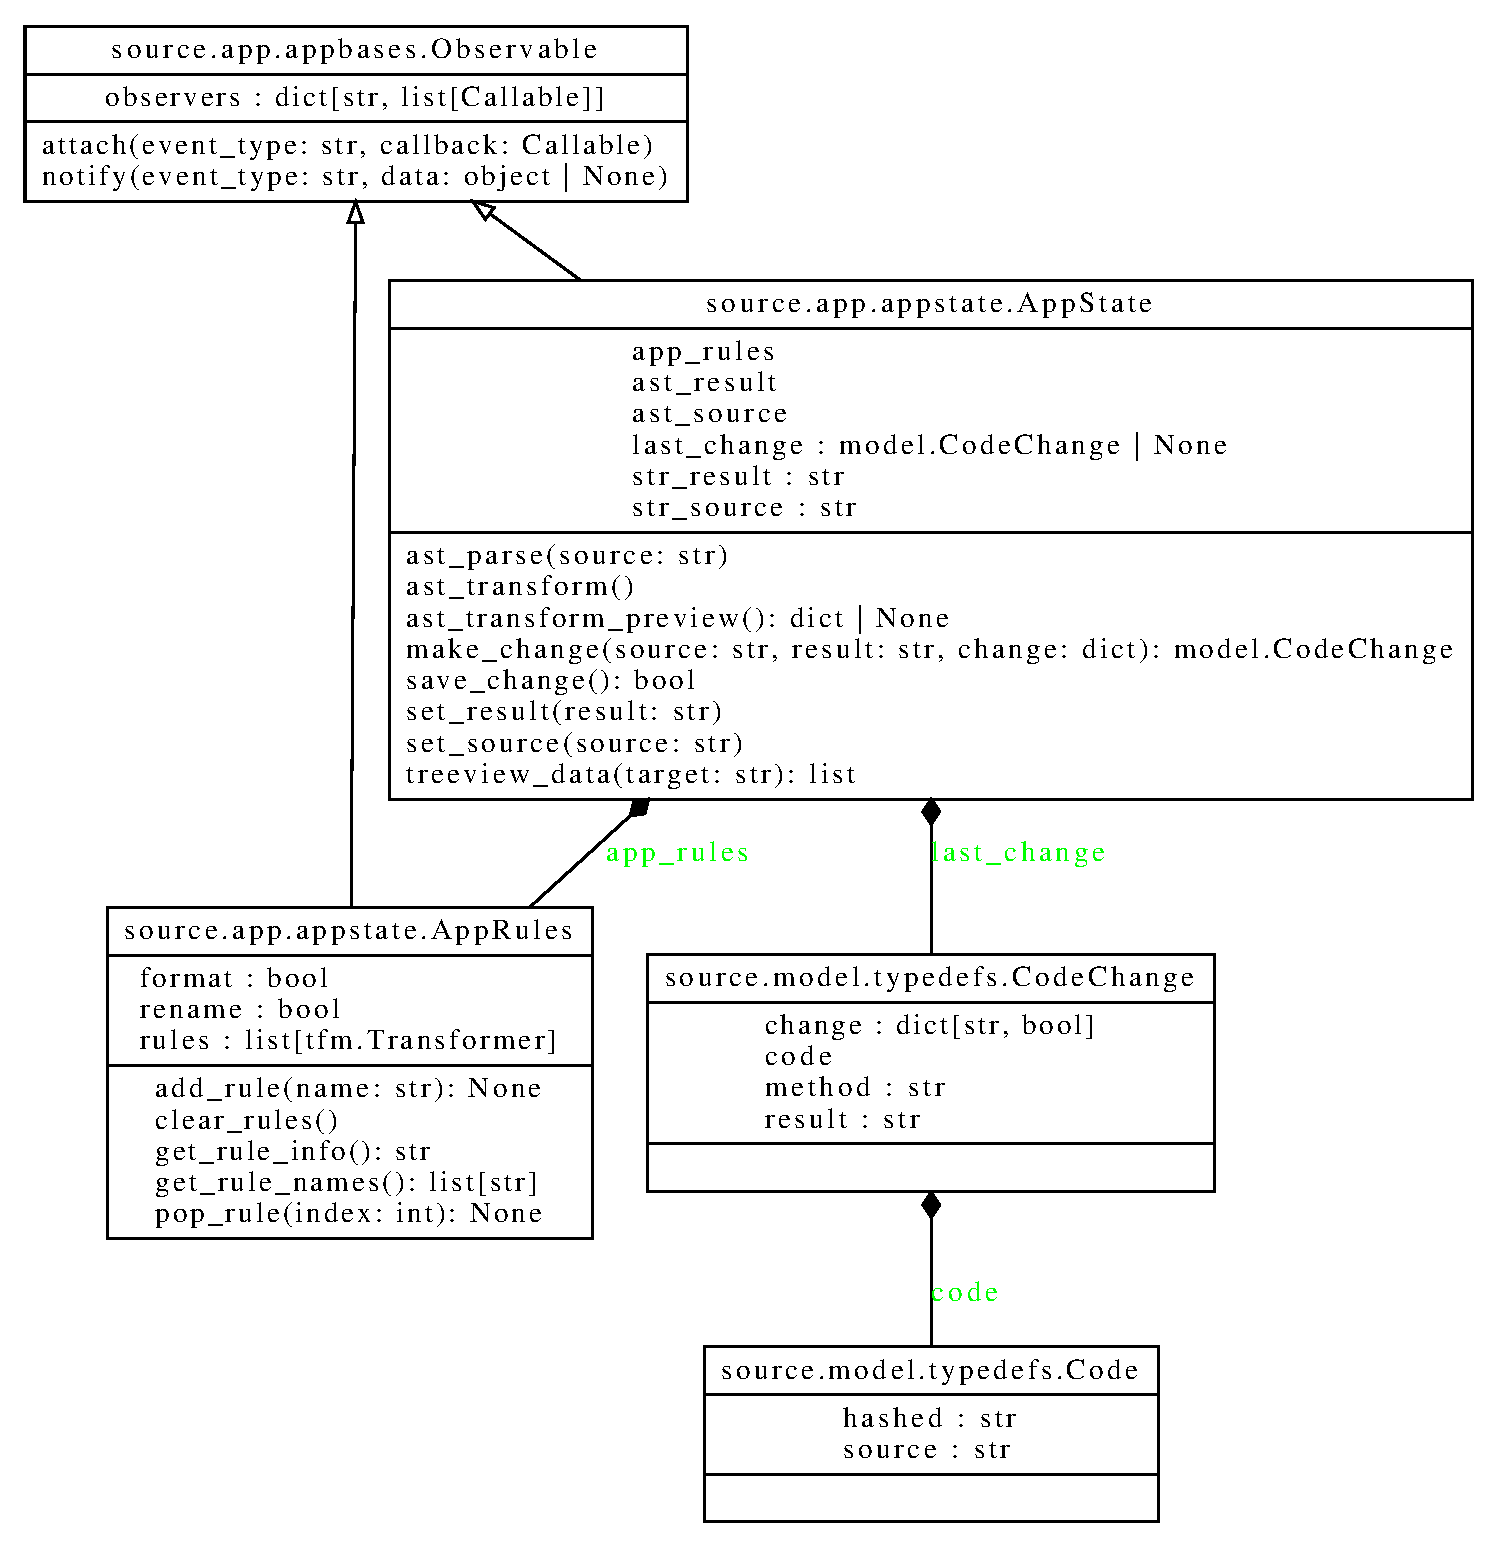
\includegraphics[width=0.9\textwidth]{images/uml/appstate.eps}
	\caption{Állapotmodell és kapcsolódó osztályok UML diagramjai}
\end{figure}

Az alkalmazás egy állapotát a bemeneti és kimineti AST-k, az ezekből generált kódok,
az átalakításért felelő szabályok listája, és az utolsó átalakítás írják le.

Az AST-k és a belőlük generált kódok az \emph{AppState} osztály példány szintű változói.
Ezeken kívül az állapotmodell az \emph{AppRules} és a \emph{CodeChange} osztályok egy-egy
példányát
is tartalmazza, ezek rendre az átalakításért felelő szabályokat és az utolsó átalakítást
tárolják.

Az \emph{AppRules} a szabályok állapotát modelezi, szintén az \emph{Observable}-ből
származik.
Ez az osztály tartalmazza a kiválasztott szabályokat a \emph{rules} listában,
a \emph{format} és \emph{rename} bool-okkal pedig azt tárolja, hogy az átalakított
kódot kell-e formatálni és az átnevezéseket végre kell-e hajtani.

Az utolsó valid átalakítást a \emph{CodeChange} osztály egy példánya tárolja.
Ahogy azt az előző szekcióban is említettem ezzel az osztállyal,
lehet kimenteni az átalakítást az adatbázsiba.

Az \emph{AppState} metódusai segítségével változtathatjuk a modellt.
A metódusok az AST-k átalakítását és az utolsó átalakítás mentését valósítják meg,
ezek a metódusok váltják ki a modellel kapcsolatos eseményeket is.

\subsection{Nézetek}

Az alkalmazás grafikus felhasználói felületének megvalósításához
a Python-ban alapból megtalálható
\emph{tkinter} könyvtárt használom, amit az erre építő \emph{ttkbootstrap} könyvtárral
egészítek ki.
A felhasználói felület forráskódja az \emph{app.views} csomagban és az \emph{app.widgets}
modulban található.

A \emph{tkinter} könyvtárban a GUI elemeket widget-eknek hívják,
az \emph{app.widgets} az ilyen widget-eket definiálja, például
a Python szintaxis kiemelést támogató szövegdobozt vagy az AST-ket ábrázoló
fa-nézeteket.

Az applikáció komplexebb nézeteinek definíciói az \emph{app.views} csomagban vannak.
Ezek a nézetek szintén widget-ek, de az \emph{app.widgets} widget-eivel ellentétben
egy kontrollerel rendelkeznek, amit a modellel való kommunikációhoz használnak
(az \emph{app.widgets} widget-ei nem férnek hozzá a modellekhez).

Az alkalmazásnak három kontrollerrel rendelkező widgete van,
ezek osztálydiagrammjait az alábbi ábrán láthatjuk.

\begin{figure}[H]
	\centering
	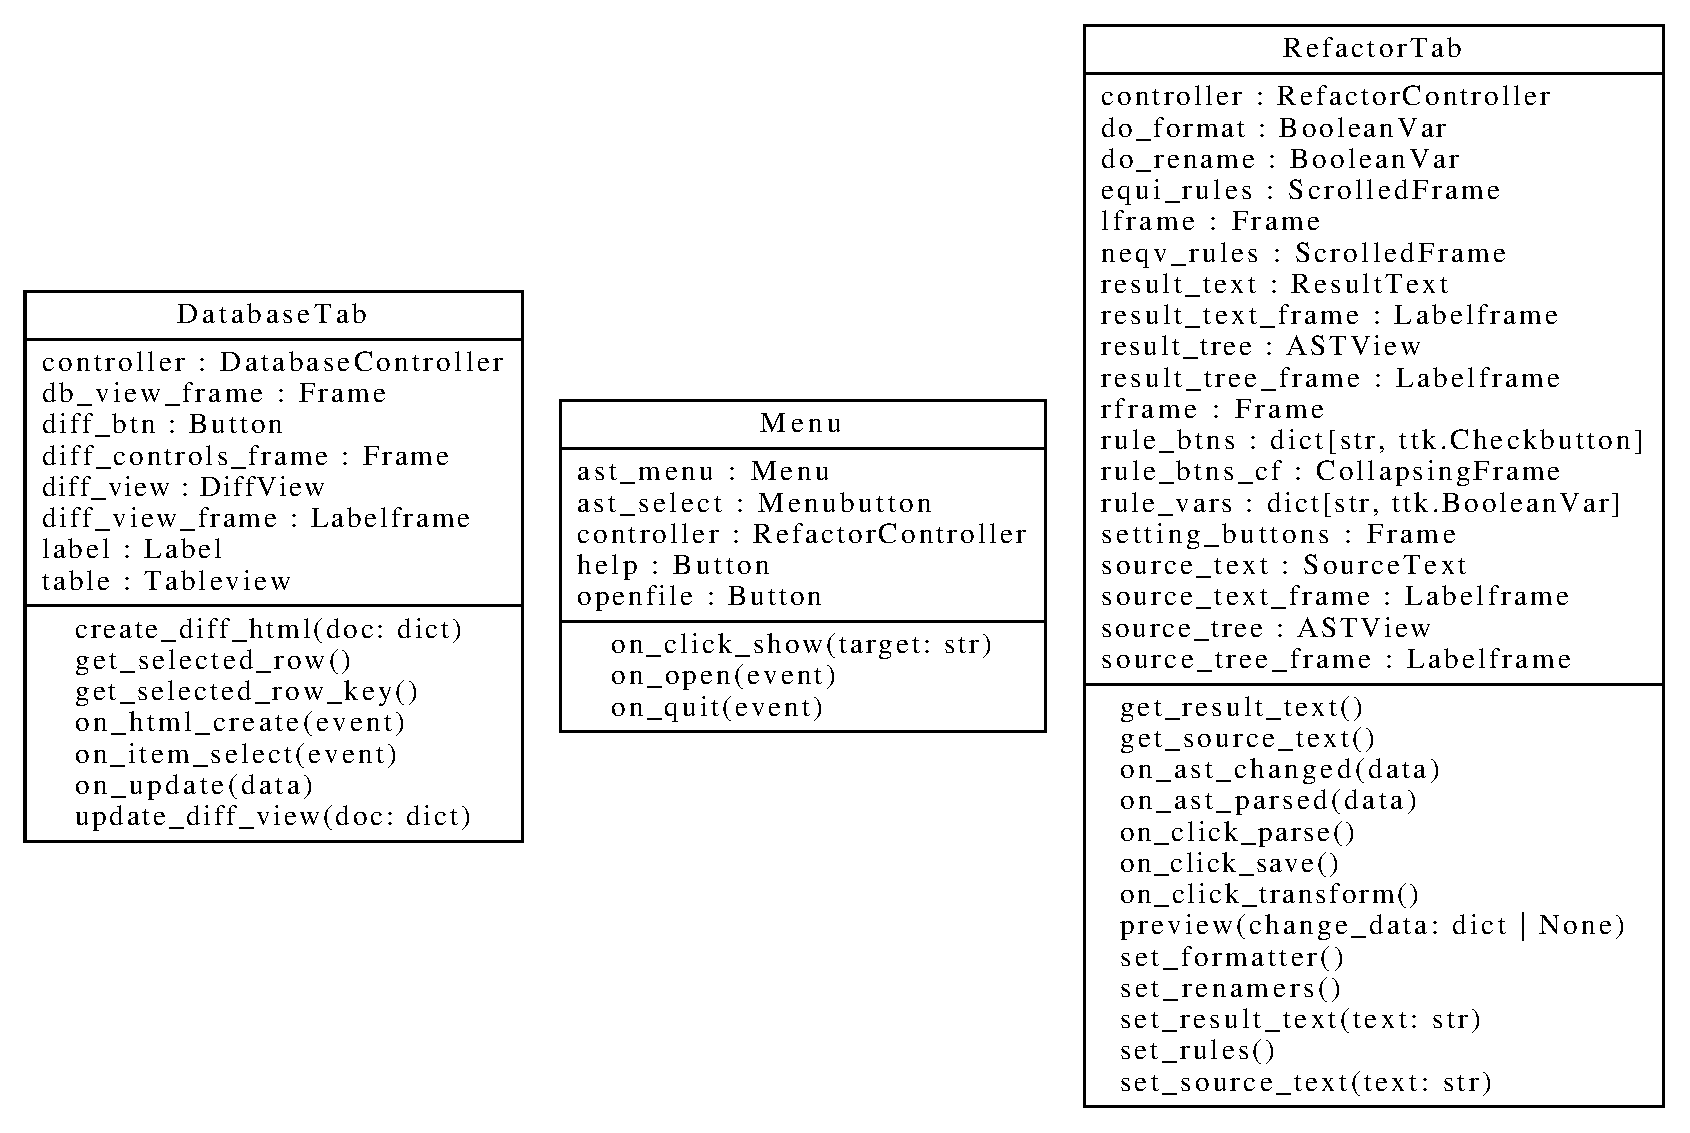
\includegraphics[width=0.9\textwidth]{images/uml/views.eps}
	\caption{\label{fig:views}A nézetek osztálydiagrammjai}
\end{figure}

\subsection{Kontrollerek}

A kontrollerek feladata a kommunikáció a modellek és nézetek között.
Csak a felhasználói felület két fő nézete (\emph{DatabaseTab} és \emph{RefactorTab})
illetve a menü nézete (\emph{Menu}) rendelkeznek kontrollerrel.

Ahogy azt a \ref{fig:views}. ábrán láthatjuk az applikációban két kontroller van.
A \emph{DatabaseController} az adatelérési modellekkel,
a \emph{RefactorController} az alkalmazás állapotmodelljével kommunikál.

\begin{figure}[H]
	\centering
	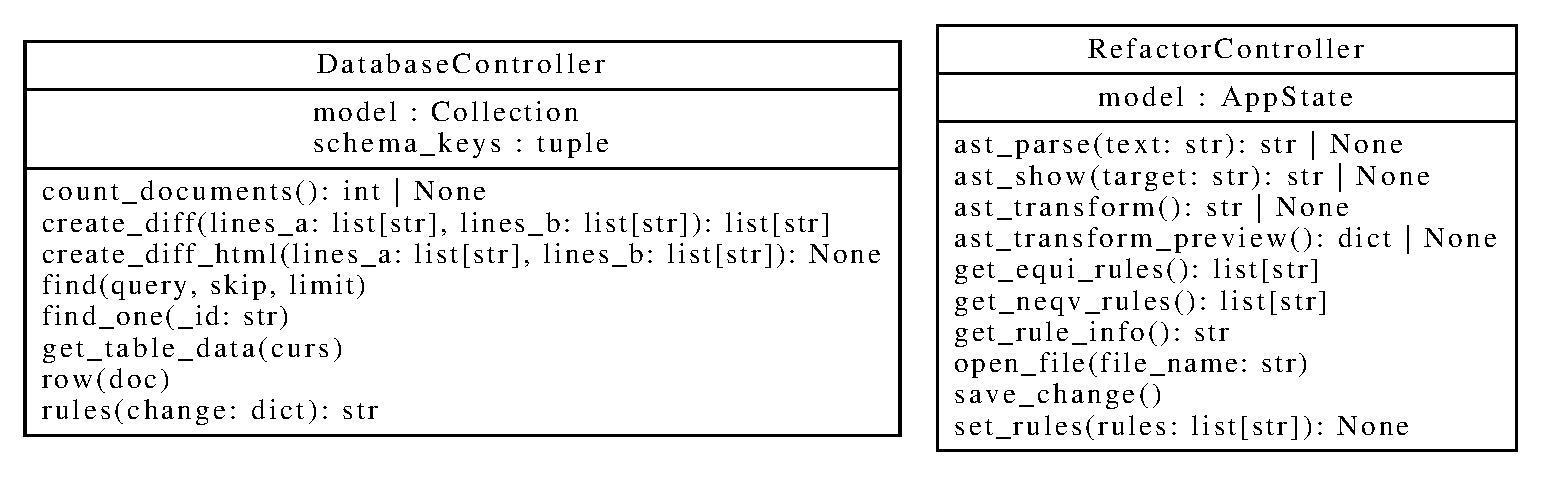
\includegraphics[width=0.9\textwidth]{images/uml/controllers.eps}
	\caption{\label{fig:controllers}A nézetek osztálydiagrammjai}
\end{figure}

Ha a nézeten olyan GUI esemény, történik aminek az eseménykezelője
a modell vagy az állapotmodell használatát igényli,
akkor az eseménykezelő a nézethez tartozó kontroller megfelelő metódusát hívja meg.
Ha az eseményhez input is tartozik (pl. egy szöveges doboz tartalma) akkor
azt is továbbítja a kontroller metódusának paraméterként.

A kontroller használja a modellt, lekérdezéseket vagy változtatásokat végez benne,
ha ezek megtörténtek a nézetet direk vagy indirekt módon frissíti.
Direkt módon frissíti, ha a modelltől kapott adatokat a nézetnek továbbítja,
ami azokkal frissül.
Ha a kontroller egy eseményt vált ki a modellben, aminek hatására a nézet frissül,
akkor indirekt frissíti.
Ezt a működést az alábbi ábrán láthatjuk.

\begin{figure}[H]
	\centering
	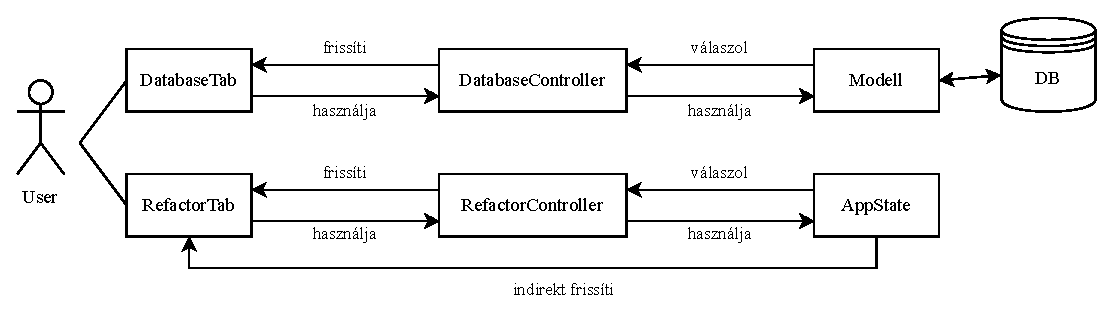
\includegraphics[width=0.9\textwidth]{images/figs/MVC.eps}
	\caption{Egy esemény kezelése az MVC architektúrában}
\end{figure}

Az alkalmazásban csak a \emph{RefactorController} végez indirekt frissítést a
\ref{subsec:appstate}. alcím alatt részletezett \emph{Observable} tervezési minta
segítségével. 

\pagebreak

\section{A \emph{transformations} csomag}
TODO

\pagebreak

\section{Tesztelés}

TODO
